\let\negmedspace\undefined
\let\negthickspace\undefined
\documentclass[journal]{IEEEtran}
\usepackage[a5paper, margin=10mm, onecolumn]{geometry}
%\usepackage{lmodern} % Ensure lmodern is loaded for pdflatex
\usepackage{tfrupee} % Include tfrupee package

\setlength{\headheight}{1cm} % Set the height of the header box
\setlength{\headsep}{0mm}     % Set the distance between the header box and the top of the text

\usepackage{gvv-book}
\usepackage{gvv}
\usepackage{cite}
\usepackage{amsmath,amssymb,amsfonts,amsthm}
\usepackage{algorithmic}
\usepackage{graphicx}
\usepackage{textcomp}
\usepackage{xcolor}
\usepackage{txfonts}
\usepackage{listings}
\usepackage{enumitem}
\usepackage{mathtools}
\usepackage{gensymb}
\usepackage{comment}
\usepackage[breaklinks=true]{hyperref}
\usepackage{tkz-euclide} 
\usepackage{listings}
% \usepackage{gvv}                                        
\def\inputGnumericTable{}                                 
\usepackage[latin1]{inputenc}                                
\usepackage{color}                                            
\usepackage{array}                                            
\usepackage{longtable}                                       
\usepackage{calc}                                             
\usepackage{multirow}                                         
\usepackage{hhline}                                           
\usepackage{ifthen}                                           
\usepackage{lscape}
\begin{document}

\bibliographystyle{IEEEtran}
\vspace{3cm}

\title{NCERT-8.1.10}
\author{EE24BTECH11023 - RASAGNA}

% \maketitle
% \newpage
% \bigskip
{\let\newpage\relax\maketitle}

\renewcommand{\thefigure}{\theenumi}
\renewcommand{\thetable}{\theenumi}
\setlength{\intextsep}{10pt} % Space between text and floats


\numberwithin{equation}{enumi}
\numberwithin{figure}{enumi}
\renewcommand{\thetable}{\theenumi}
\textbf{Question:}
Find the area bound by the curve $x^2=4y$ and the line $x=4y-2$.

\textbf{Solution:}
The given parabola equation can be expressed as
\begin{align}
    g\brak{\vec{x}}= \vec{x}^{\top}\vec{V}\vec{x}+2\vec{u}^{\top}\vec{x}+f=0,
\end{align}
where,
\begin{align}
    \vec{V}=\myvec{1 & 0 \\ 0 & 0 }, \vec{u}=\myvec{0\\ {-2}}, f=0.  
\end{align}
\begin{align}
  \myvec{x&y}\myvec{1&0\\0&0}\myvec{x\\y}+2\myvec{0 & -{2}}\myvec{x\\y}+0=0
\end{align}
Given line equation can be expressed as,
\begin{align}
    x=h+km
\end{align}
where,
\begin{align}
    \vec{h}=\myvec{0\\ \frac{1}{2}},\vec{m}=\myvec{1\\ \frac{1}{4}}
\end{align}
Intersection of a line and a conic is given by,
\begin{align}
  \kappa_i=\frac{-\vec{m}^{\top}\brak{\vec{Vh}+\vec{u}}\pm\sqrt{\sbrak{\vec{m}^{\top}\brak{\vec{Vh}+\vec{u}}}^2-g\brak{h}\brak{\vec{m}^{\top}\vec{Vm}}}}{\vec{m}^{\top}\vec{Vm}}
\end{align}
simplifying and substituting the values,\\
we get,
\begin{align}
    k_1={-1},k_2=2
\end{align}
By substituting $k_1$ and $k_2$ values in equation \brak{0.4},we get the points of intersection as, $\myvec{-1\\\frac{1}{4}}, \myvec{2\\1}$
Equation for area enclosed is given by,
\begin{align}
    A = \int_{-1}^2 \left| \frac{x + 2}{4} - \frac{x^2}{4} \right| \, dx
\end{align}
\textbf{Theoritical Solution}
\begin{align}
A &= \int_{-1}^2 \left| \frac{x + 2}{4} - \frac{x^2}{4} \right| \, dx \\
&= \frac{1}{4} \int_{-1}^2 \left( x + 2 - x^2 \right) \, dx.
\end{align}
\begin{align}
A &= \frac{1}{4} \left[ \frac{x^2}{2} + 2x - \frac{x^3}{3} \right]_{-1}^2.
\end{align}
\begin{align}
A &= \frac{1}{4} \bigg[ \bigg( \frac{2^2}{2} + 2(2) - \frac{2^3}{3} \bigg) - \bigg( \frac{(-1)^2}{2} + 2(-1) - \frac{(-1)^3}{3} \bigg) \bigg] \\
&= \frac{1}{4} \bigg[ \bigg( 2 + 4 - \frac{8}{3} \bigg) - \bigg( \frac{1}{2} - 2 + \frac{1}{3} \bigg) \bigg]\\
&=\frac{9}{8}
\end{align}
\textbf{Computational Solution}
To calculate the area under the curve $y_x$ from $x = x_0$ to $x = x_n$, we approximate it using trapezoidal strips of small areas. The $x$-axis is discretized into points $x_0, x_1, x_2, \dots, x_n$, such that the spacing between consecutive points is equal, with a step size of $h$. 
The total area, as the sum of all trapezoidal areas, is given by:
\begin{align}
  A&=\frac{1}{2}h\brak{y\brak{x_1}+y\brak{x_0}}+ \frac{1}{2}h\brak{y\brak{x_2}+y\brak{x_1}}+\dots+\frac{1}{2}h\brak{y\brak{x_n}+y\brak{x_{n-1}}}\\
  &=h\sbrak{\frac{1}{2}\brak{y\brak{x_0}+y\brak{x_n}}+ y\brak{x_1}+\dots+y\brak{x_{n-1}}}
\end{align}
Let $A\brak{x_n}$ be the area enclosed by the curve $y\brak{x}$ from $x=x_0$ to $x=x_n$, $\brak{x_0, x_1, \dots x_n}$ be equidistant points with step-size $h$.
\begin{align}
  A\brak{x_n+h}=A\brak{x_n}+\frac{1}{2}h\brak{y\brak{x_n+h}+y\brak{x_n}}
\end{align}
We can iterate till we get required area.
Discretizing the steps, making $A\brak{x_n}=A_n, y\brak{x_n}=y_n$,
\begin{align}
 A_{n+1}=A_n+\frac{1}{2}h\brak{y_{n+1}+y_n}
\end{align}
Using first principle of derivative,$y_{n+1}=y_n+hy^{\prime}_n$
\begin{align}
  A_{n+1}&=A_n+\frac{1}{2}h\brak{\brak{y_{n}+hy^{\prime}_n}+y_n}\\
  A_{n+1}&=A_n+\frac{1}{2}h\brak{2y_n+hy^{\prime}_n}\\
  A_{n+1}&=A_n+hy_n+\frac{1}{2}h^2y^{\prime}_n\\
  x_{n+1}&=x_n+h
\end{align}
In the given question, $y_n=x_n+2-x_n^2$ and $y^{\prime}_n=1-2x_n$.\\
General Difference Equation is given by,
\begin{align}
  A_{n+1}&=A_n+hy_n+\frac{1}{2}h^2y^{\prime}_n\\
  &=A_n+h\brak{x_n+2-x_n^2}+\frac{1}{2}h^2\brak{1-2x_n}\\
  &=A_n+x_n\brak{h-h^2}-x_n^2\brak{h}+\frac{h^2}{2}+2h\\
  x_{n+1}&=x_n+h
\end{align}
We should iterate till $x_n=2$ to get the required area.\\
The obtained theoritical solution is 1.125 sq.units.\\
The computational solution is 1.1249988750000004sq.units.\\
\begin{center}
    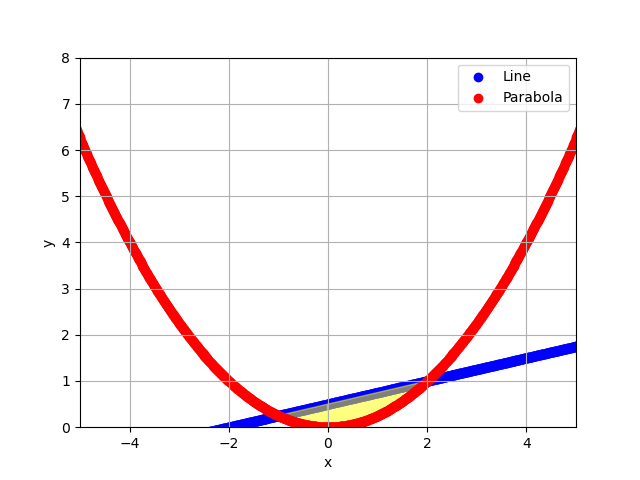
\includegraphics[width=0.75\columnwidth]{figs/figss.png}
\end{center}
\end{document}